\section{Introduction}
Literature research is one of the most essential task to accomplish in a regular scientific research process. However, it's usually a complex and time-consuming task. That's why we have implemented \textit{Icecite}, a fully web-based research manager aimed to automatize and to facilitate the necessary steps of a \textit{digital} literature research process. \textit{Digital} means that Icecite concentrates on managing digital literary materials, namely scientific research papers provided as PDF files.

One of the core features of Icecite is the automatic identification of both, the metadata (title, author(s), year, journal, etc.) and the bibliographic references in given research papers. Our approach splits the identification process into 2 steps. In the first step, we extract significant data from given PDF files (e.g. the titles and the entries of bibliographies). In the second step, we match each extract to the referred record of an underlying digital library (e.g. DBLP or Medline) to get the full and correct metadata fields. Our approach outperforms traditional machine learning approaches in terms of runtime and accuracy of identified data.

On the basis of the automatic identification of data, Icecite can provide an extensive set of further features, that exceeds the feature sets of existing (mainly desktop-based) software solutions.  The full feature set of Icecite includes: 
\begin{enumerate}[{(1)}]
 \setlength{\itemsep}{-2pt}
 \item Managing research papers in a personal library.
 \item Automatic identification of metadata of research papers.
 \item Automatic identification of bibliographic references of research papers.
 \item Instant search in DBLP and Medline.  
 \item Instant (fulltext-)search in personal collection of research
 papers.
 \item Importing document from digital libraries into the library with a single click.
 \item Automatic search for PDF files, providing fulltexts of research papers.
 \item Reading \& Annotating of PDF files in browser.
 \item Tagging of  research papers with keywords.
 \item Offline usability.
 \item Synchronization of the library data (metadata, references, PDF files, annotations).
 \item Sharing of the library data with other member nearly in real-time.
 \item Fully web-based and easy-to-use user interface
\end{enumerate}
In the following, we will give an overview how the listed features act together to form the general structure of Icecite and how they support the following most essential tasks of a proper literature research process.
%Each listed feature contributes to improve the experiences on doing literature research. To substantiate this, we now introduce the most essential tasks of a proper literature research process and clarify, how they are automatized by Icecite.

\paragraph{Organize collections of research papers} 
\noindent
Doing scientific literature research usually implies the need to manage a set of collected literary materials, i.e. digital research papers provided as PDF files as mentioned above.

The collection may consist of locally stored files or bookmarks to the locations of files in web, or both. Depending on the size of the collection, keeping a consistent structure on naming the files are recommended, in order to keep track of them. However, finding proper filenames and renaming the files are annoying and time-consuming tasks. 

\begin{figure*}[!ht]
  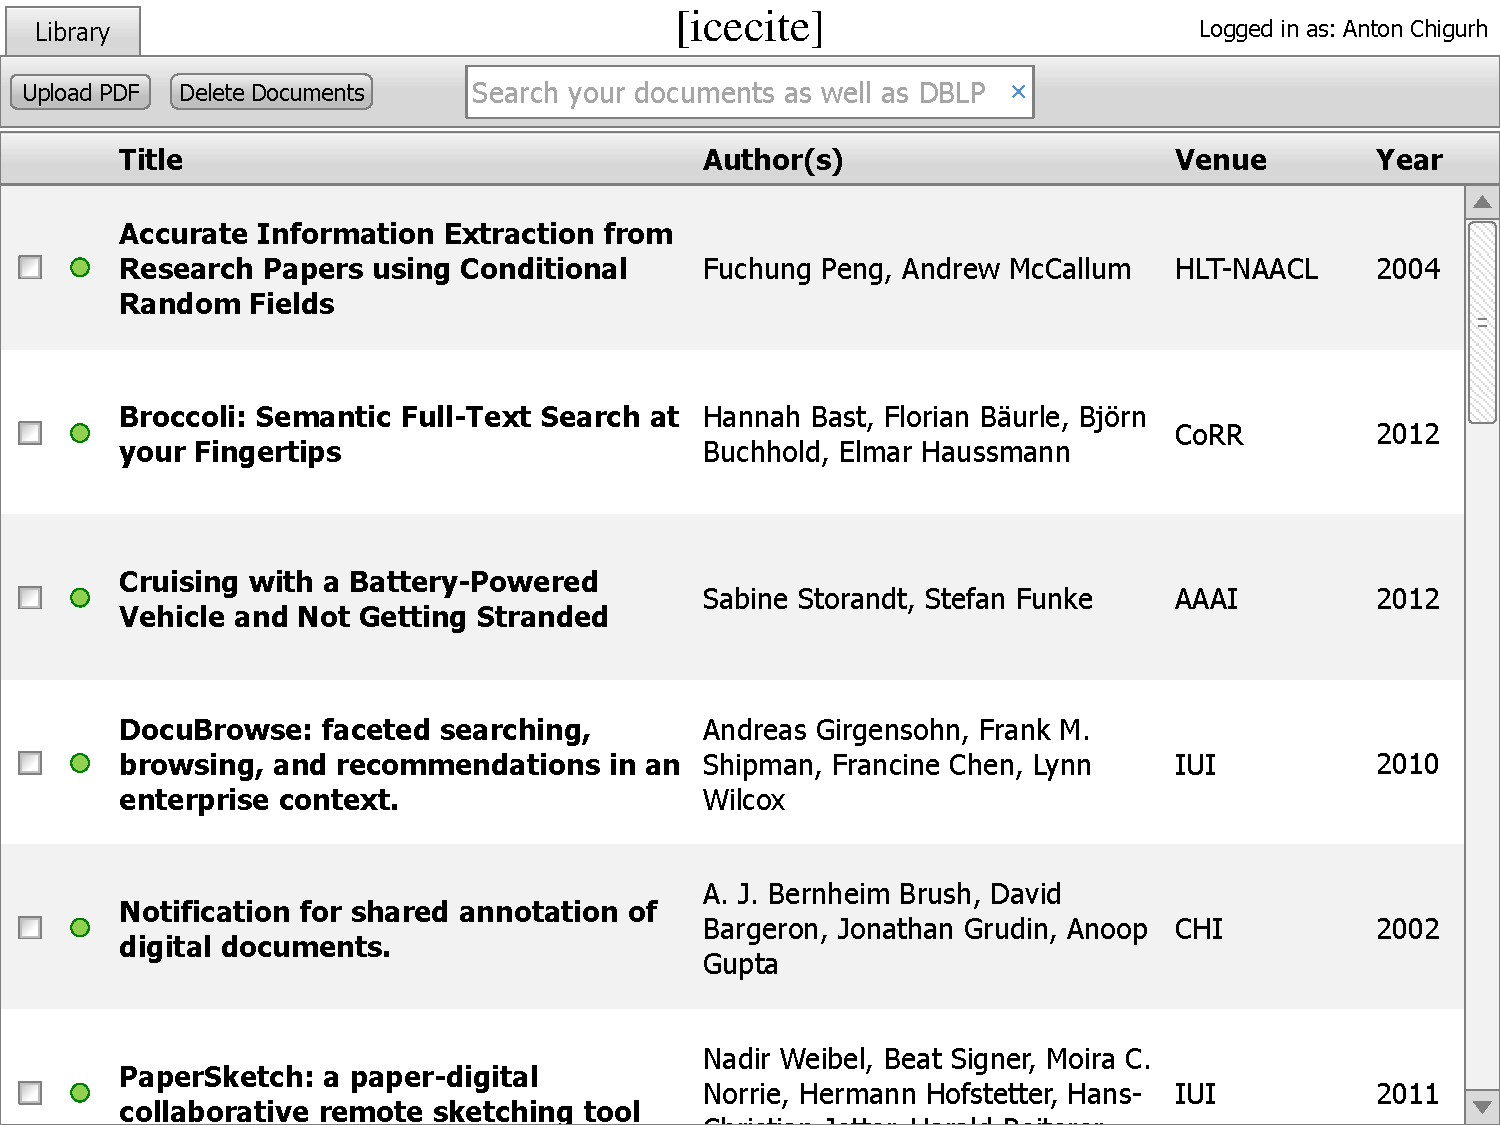
\includegraphics[width=\textwidth]{./figures/libraryview}
  \caption{A screenshot of the \textit{library view} in Icecite. Each entry of library is listed with the following metadata fields: title, author(s), conference and year of publication. The checkbox besides each entry exists, to select the entry for deletion (the deletion is actually done by clicking the button \textit{Delete Documents} in the upper left).  The small bullet to the left of the title of each entry displays the status of entry (a \textit{green} bullet means, that the full metadata were found for entry). On clicking the button \textit{Upload PDF}, you can add a locally stored PDF file to library. The needed metadata will be computed automatically then. You can type in a search query into the search field (located to the right of the \textit{Delete Document} button), to search in own library as well as in the digital library \textit{DBLP}. On clicking an entry of search result, it will be added to library. In contrast, on clicking an entry of library, user is forwarded to the \textit{document view} (cf. Figure \ref{fig:screenshot_documentview}).}
  \label{fig:screenshot_libraryview}
\end{figure*}

Icecite eliminates these steps entirely by holding all the collected research papers (\textit{documents}) in a personal \textit{library}. A library is placed in the \textit{library view} of Icecite (shown in figure \ref{fig:screenshot_libraryview}, consider the caption below the figure for a detailed explanation of each UI-element). On adding a document to the library, its metadata and its bibliographic references are identified automatically due to the features (1)+(2). Because the metadata are used to describe the document uniquely, there is no need anymore to name files manually. The identified references of a document are placed next to the PDF file in the \textit{document view} (shown in figure \ref{fig:screenshot_documentview}), that is accessible via clicking a document in the library view. A more detailed discussion about our approach of automatic identification of metadata and bibliographic references can be found in section \ref{sec:extraction}.    

Although Icecite is web-based, all library data (metadata, PDF files, etc.) are stored locally on client's filesystem. That's why some features of Icecite can be used even in case of offline mode, e.g. browsing the library, annotating PDF files or load PDF files into the library (certainly without automatic identification of metadata and references). It can be achieved by using features of the html5 standard, as described in section \ref{sec:html5}.	

Additionally, the library data are synchronized periodically with the server to (1) access them from any location and (2) share them with other users for collaboration. The mechanism of data synchronization is described in section \ref{sec:sync}.

\begin{figure*}[ht]
  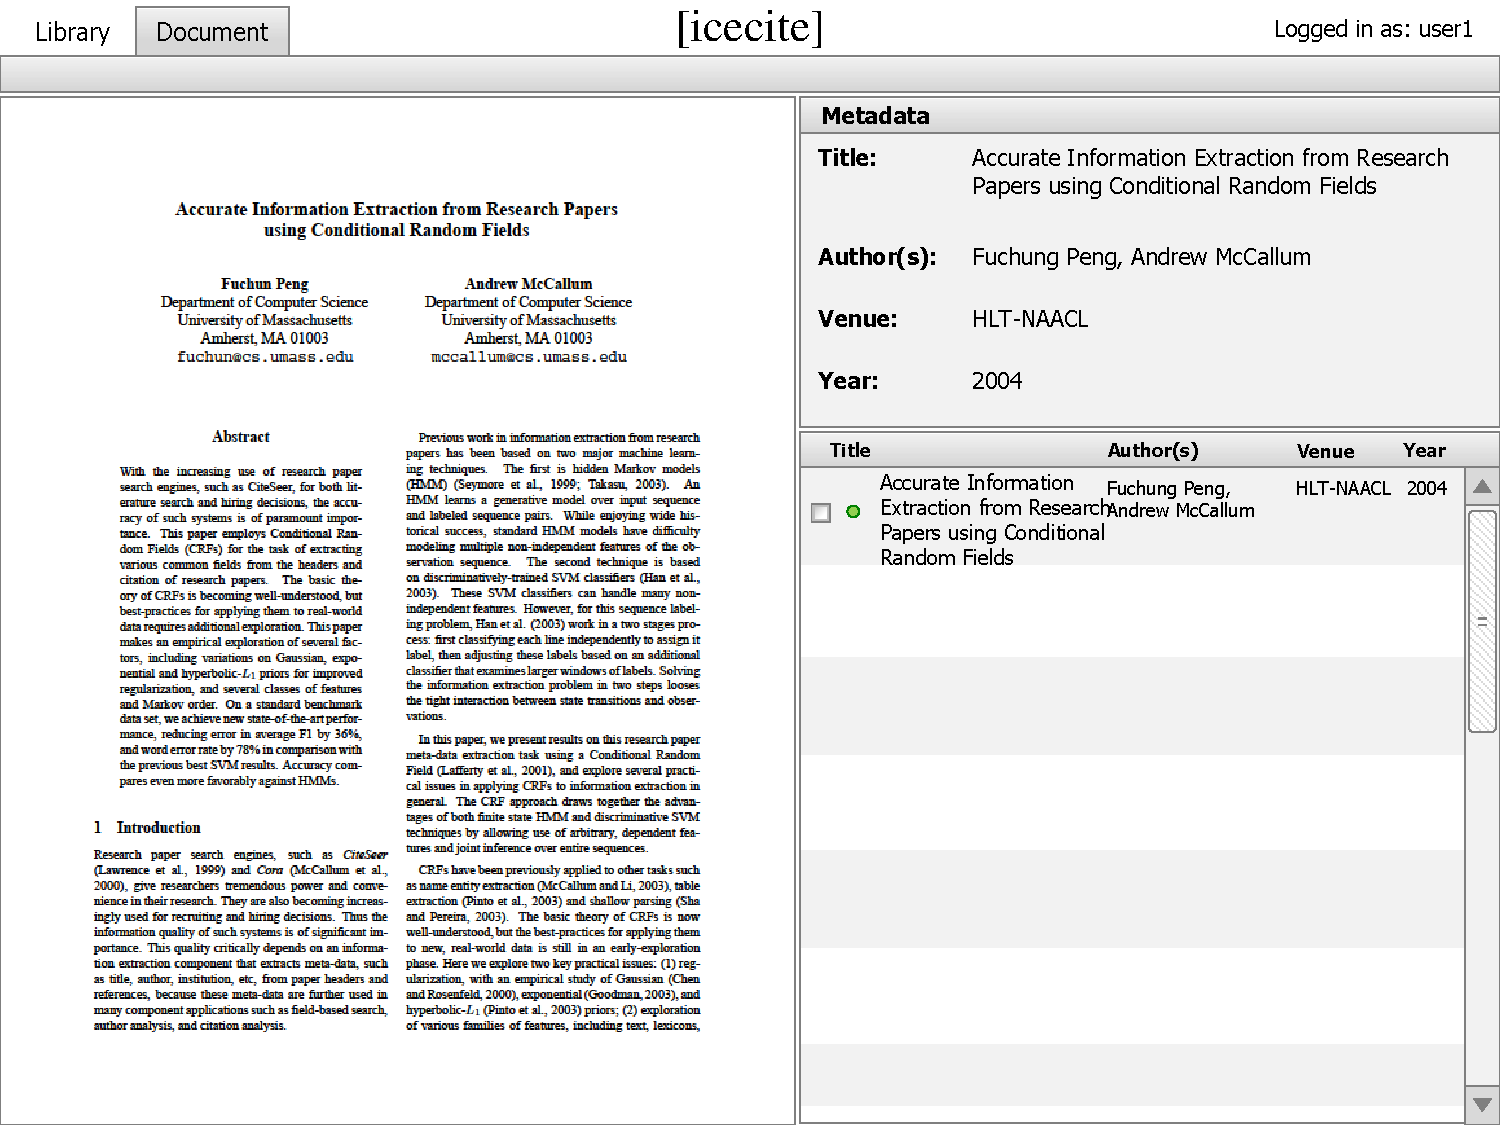
\includegraphics[width=\textwidth]{./figures/documentview}
  \caption{A screenshot of the \textit{document view} in Icecite. It shows both, the pdf file of research paper and the metadata of the paper and its references. Here you can read, annotate and comment the pdf file (you can turn the pdf into fullscreen-mode to hide the metadata to the right) and study the metadata of references. The entries of references list are of the same design as the entries in the \textit{library view} (cf. figure \ref{fig:screenshot_libraryview}). Again, on clicking an entry of references, you can add it to library, to read, annotate and share it and to study its references.}
  \label{fig:screenshot_documentview}
\end{figure*}

\paragraph{Searching for topic-related research papers} 
\noindent
In order to explore topic-related research papers and to extend the personal collection with them, generally the following 4 sources can be consulted:

\par\medskip\noindent
\textit{(S1)} Digital libraries, such as \textit{DBLP} or \textit{Medline}.
\par\smallskip\noindent
\textit{(S2)} The web, such as publisher websites (like \textit{ACM}, \textit{IEEE}, \textit{Springerlink}, etc.)
\par\smallskip\noindent
\textit{(S3)} Bibliographies from already known research papers.
\par\smallskip\noindent
\textit{(S4)} Personal recommendations.
\medskip

The listed sources differ from each other in the amount of provided data. While the sources \textit{(S1)} and \textit{(S2)} may provide (links to) PDF files of research papers, the sources \textit{(S3)} and \textit{(S4)} usually don't (but only parts of metadata fields). Hence, in case of sources \textit{(S3)} and \textit{(S4)}, extra effort is needed to retrieve the PDF files (e.g. by consulting the source \textit{(S1)} or \textit{(S2)} in addition). However, the invested time and effort may be in vain, if a file isn't fetchable, because it isn't available in general or the access to it is restricted and only available to licensees. 

Due to the automatic identification of bibliographic references (2), the instant search in DBLP and Medline (3) and the automatic search for PDF files (5), Icecite speeds up the whole process of fetching topic-related research papers substantially. 
\TODO{Eliminate this listing, and reuse it in infrastructure section} 
Generally, there are three ways to add a new document to the library: 

\par\medskip\noindent
\textit{(ADD 1)} Upload a PDF file to the library.
\par\medskip\noindent
\textit{(ADD 2)} Click an entry in the reference list of a selected document in the document view.
\par\medskip\noindent
\textit{(ADD 3)} Type a search query into the search field of the library view to browse for any entries in a digital library (DBLP or Medline). Click a record of the search result.
\medskip

Variant \textit{(ADD 1)} is followed directly by the automatic identification of the metadata and the bibliographic references of the research paper given by the uploaded PDF file. Once all the metadata and references are retrieved, the document is added to the library.

In contrast, variants \textit{(ADD 2)} and \textit{(ADD 3)} are firstly followed by the automatic search for a PDF file, that contains the fulltext of the clicked record in the references list (resp. the search result). The PDF file is located in the web via the metadata, which were retrieved on the references identification (resp. via the metadata provided by the digital library). Once the PDF file was found, the further processing is similar to that for variant \textit{(ADD 1)} as described above. See section \ref{sec:search} for a more detailed discussion of the search in digital libraries and the automatic search for PDF files.

\paragraph{Reading research papers} 
\noindent
While reading the PDF file of a research paper, it's quite common, to highlight some text passages and to make some notes to it. With Icecite, PDF files can be read online, if there is a proper browser plugin is installed to display the PDF files in the browser and can be even annotated, if the plugin of Adobe Acrobat is used. On implementing this feature, we have paid attention to use \textit{native}\footnote{With native annotations we mean those annotations, which conform to the official PDF specifications} annotations. This ensures, that the annotations are identified as such not only within Icecite, but also in various external PDF viewers. See the detailed desciption of this feature in section \ref{sec:annotations}, why this intention isn't trivial to achieve.

\paragraph{Collaborate in groups} 
\noindent
On collaborating in (research-)groups to review some research papers together, many individual annotations are produced. Icecite is able to combine the individual annotations made to a PDF file to get a general conclusion. The data of library can be shared with other users nearly in real-time. So, once the set of documents and annotations in shared libraries was changed by a member of group, the changes are displayed to the other members instantly. See section \ref{sec:sync} for a more detailed discussion of this feature. \\

In section \ref{sec:related_work}, we will introduce some applications, that are related to Icecite. There are both, desktop-based and web-based applications, although existing desktop-based applications typically provide larger feature sets than existing web-based applications. We will compare the features of both types with those of Icecite.
However, desktop-applications have some drawbacks... \\
\TODO{list drawbacks of desktop applications.}\\
\TODO{Present results of experiments}.\\
\TODO{Present results of user study}.

At the end of this introduction, we want to clarify, that the contribution of this paper is the overall design of Icecite and the basic ideas for each of the individual components of the system. Consider, that these components are complex problems each on their own and can not be discussed in all details in this paper. However, in section \ref{sec:futurework} we will give you an idea, how the various components can be optimized on future research.